%&latex
\documentclass[12pt]{article}
\usepackage{authblk}
\usepackage{amsmath}
\usepackage{amssymb}
\usepackage{booktabs}
\usepackage{graphicx}
\usepackage{psfrag,epsf}
\usepackage{enumerate}
\usepackage{natbib}
\usepackage{url} % not crucial - just used below for the URL
\usepackage{comment}
\RequirePackage[colorlinks,citecolor=blue,urlcolor=blue]{hyperref}
\usepackage{setspace}

\newcommand{\jy}[1]{\textcolor{red}{JY: #1}}
\newcommand{\eds}[1]{\textcolor{blue}{(EDS: #1)}}
\newcommand{\mc}[1]{\textcolor{green}{(MC: #1)}}
\newcommand{\xz}[1]{\textcolor{cyan}{(XZ: #1)}}

\allowdisplaybreaks

\usepackage[pagewise]{lineno}
\linenumbers*[1]
% patches to make lineno work better with amsmath
\newcommand*\patchAmsMathEnvironmentForLineno[1]{%
        \expandafter\let\csname old#1\expandafter\endcsname\csname 
        #1\endcsname
        \expandafter\let\csname oldend#1\expandafter\endcsname\csname 
        end#1\endcsname
        \renewenvironment{#1}%
        {\linenomath\csname old#1\endcsname}%
        {\csname oldend#1\endcsname\endlinenomath}}%
\newcommand*\patchBothAmsMathEnvironmentsForLineno[1]{%
        \patchAmsMathEnvironmentForLineno{#1}%
        \patchAmsMathEnvironmentForLineno{#1*}}%
\AtBeginDocument{%
        \patchBothAmsMathEnvironmentsForLineno{equation}%
        \patchBothAmsMathEnvironmentsForLineno{align}%
        \patchBothAmsMathEnvironmentsForLineno{flalign}%
        \patchBothAmsMathEnvironmentsForLineno{alignat}%
        \patchBothAmsMathEnvironmentsForLineno{gather}%
        \patchBothAmsMathEnvironmentsForLineno{multline}%
}

\pdfminorversion=4
% NOTE: To produce blinded version, replace "0" with "1" below.
\newcommand{\blind}{0}

% DON'T change margins - should be 1 inch all around.
\addtolength{\oddsidemargin}{-.5in}%
\addtolength{\evensidemargin}{-.5in}%
\addtolength{\textwidth}{1in}%
\addtolength{\textheight}{1.3in}%
\addtolength{\topmargin}{-.8in}%


\begin{document}

%\bibliographystyle{natbib}

\def\spacingset#1{\renewcommand{\baselinestretch}%
{#1}\small\normalsize} \spacingset{1}


%%%%%%%%%%%%%%%%%%%%%%%%%%%%%%%%%%%%%%%%%%%%%%%%%%%%%%%%%%%%%%%%%%%%%%%%%%%%%%

\title{\bf Supplementary Material to\\
  ``Nonparametric Block Bootstrap Kolmogorov-Smirnov Goodness-of-Fit Test''
}
\if0\blind
{
  \author[1,2]{Mathew Chandy}
  \author[1]{Elizabeth D. Schifano}
  \author[1]{Jun Yan\thanks{
    The authors gratefully acknowledge the National Science Foundation (NSF).}\hspace{.2cm}}
  \author[3]{Xianyang Zhang$^{\ast}$ }
  \affil[1]{Department of Statistics, University of Connecticut}
  \affil[2]{Department of Statistics and Data Science, University of California, Los Angeles}
  \affil[3]{Department of Statistics, Texas A\&M University}
  \maketitle
} \fi

\if1\blind
{
  \bigskip
  \bigskip
  \bigskip
  \author{Anonymous Author}
} \fi

\maketitle

\section{Comparison of Two Bias Corrections}

A heuristic justification for the $K_n(x)$ bias correction term was
provided in the main manuscript. It may also help to demonstrate
empirically that this the block bootstrap KS test with the $K_n$ bias
correction holds its size at least as well as the block boostrap KS
test with the \citet{babu2004goodness} bias correction and is at
least as powerful. For this reason, we conducted a simulation study
with parameter settings identical to the main study in the paper
except for the choice of bias correction.

\begin{figure}[tbp]
  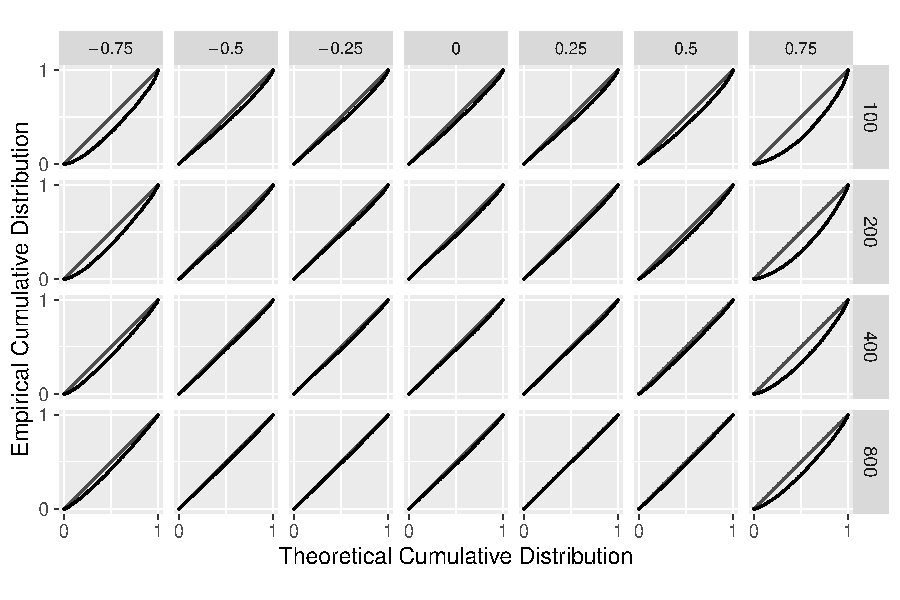
\includegraphics[width = .9\textwidth]{figures/normal_C_n}
  \centering
  \vspace{-10pt}
  \caption{Q-Q plots of the p-values testing that a time series
    have marginal normal distribution with true data generating distribution
    being $N(8,8)$ when using \citet{babu2004goodness}'s bias correction term.}
  \label{fig:qq_n_C_n}
    \hspace{3cm}
  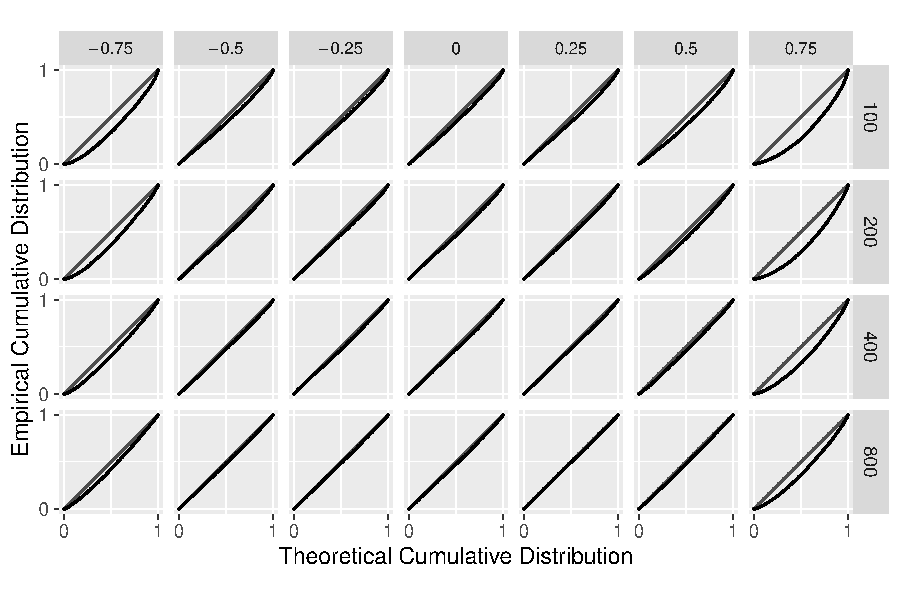
\includegraphics[width = .9\textwidth]{figures/gamma_C_n}
  \vspace{-5pt}
  \caption{Q-Q plots of the p-values testing that a time series
    have marginal gamma distribution with true data generating distribution
    being $\Gamma(8,1)$ when using \citet{babu2004goodness}'s bias correction term.}
  \label{fig:qq_g_C_n}
\end{figure}


\begin{figure}[tbp]
  \centering
  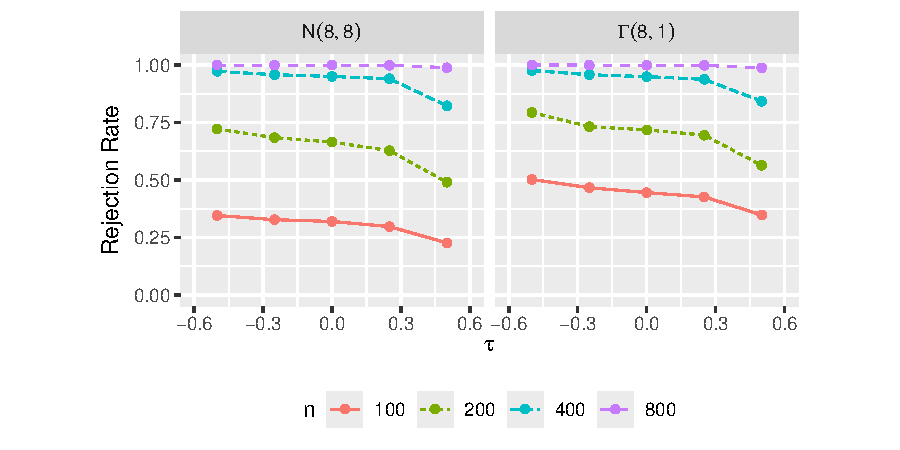
\includegraphics[scale=1]{figures/rr_C_n}
  \caption{Empirical power curve as a function of $\tau$ for
    $n \in \{100, 200, 400, 800\}$ and true marginal distribution
    $\in \{N(8,8), \Gamma(8,1)\}$, when using \citet{babu2004goodness}'s bias correction term. When the data was generated from $N(8,8)$,
    we tested for the gamma family. When the data was generated from
    $\Gamma(8,1)$, we tested for the normal family.
  }
  \label{fig:rr_C_n}
\end{figure}

Based on Figures~\ref{fig:qq_n_C_n, fig:qq_g_C_n, fig:rr_C_n}, the empirical performance is very similar under either choice of bias correction term. For practical applications, we recommend.....


\section{Block Size Selection}

The choice of block size is a key factor influencing the performance
of block bootstrap methods, particularly in settings with serial
dependence. While our main simulations used a fixed block size
$l = \lceil n^{1/3} \rceil$, the optimal block size depends on the
stength and structure of dependence \citep{hall1995blocking,
  buhlmann1999block,  politis2004automatic}. Motivated by this, we
further examined the use of an automatic block-length selection scheme
as proposed by \citet{politis2004automatic}, which aims to adaptively
choose the block size based on the data. The simulation settings
remain the same as in the study reported earlier.


% To address this, we considered  using the automatic block-length selection
% scheme for circular block bootstrap as described in Section~3.3 of
% \citet{politis2004automatic}. Unfortunately, using this setting results in
% the selection of block
% sizes that can be quite large (sometimes as large or larger than $n$), leading
% to less variation between the bootstrapped
% samples. Figures~\ref{fig:large_block}
% demonstrate that for highly temporally
% dependent samples (especially when the autocorrelation is negative),
% the block size is frequently larger than $\sqrt{n}$. For more moderate 
% positive temporal dependence, the block size may not be overly large
% as frequently. Still, even for these moderately dependent samples, the 
% block sizes are almost always larger than $l = \lceil n^{1/3} \rceil$, a setting
% which was considered optimal by \citep{buhlmann1999block}. This
% is demonstrated in Figure~\ref{fig:block_dist} with a histogram
% of the selected block sizes for the 20000 samples with $n = 800$, $\tau = 0.5$, 
% and $X_i \sim N(8, 8)$.

\begin{figure}[tbp]
  \centering
  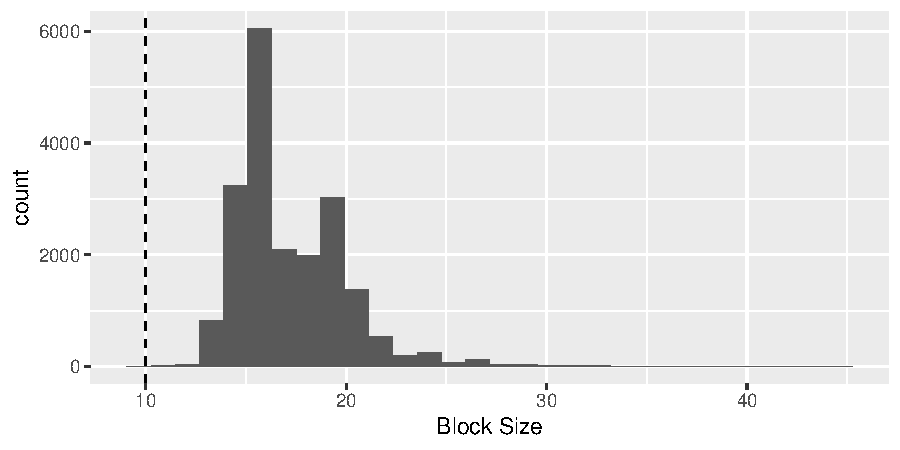
\includegraphics[scale=1]{figures/block_dist}
  \caption{Distribution of the selected block sizes using
  \citet{politis2004automatic}'s procedure applied to 20000 length-800 time 
  series with
    Kendall's $\tau = 0.5$ data generating distribution $N(8,8)$. The vertical
    dashed line is $l = \lceil n^{1/3} \rceil$ for $n = 800$, which is equivalent 
    to 10.
  }
  \label{fig:block_dist}
% \end{figure}


% \begin{figure}[tbp]
  \centering
  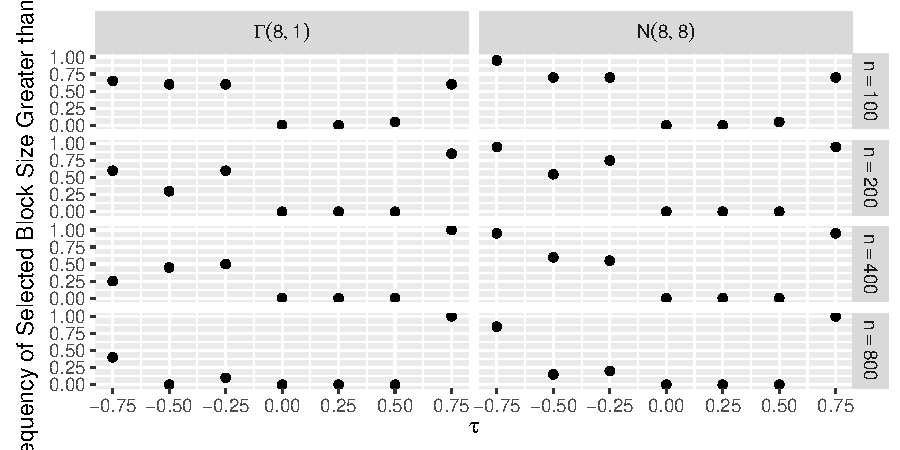
\includegraphics[scale=1]{figures/large_block}
  \caption{Proportion of selected block sizes using the method of
  \citet{politis2004automatic} that are larger than
    $\sqrt{n}$ for $n \in \{100, 200, 400, 800\}$,
    $\tau \in \{-0.75, -0.50, -0.25, 0, 0.25, 0.50, 0.75\}$, and true
    marginal distribution $N(8,8)$ and $\Gamma(8,1)$.
  }
  \label{fig:large_block}
\end{figure}

Automatic block size selection tends to yield larger block sizes than our
fixed choice $l = \lceil n^{1/3} \rceil$, as expected, but under strong
negative or very strong positive dependence it systematically produces
block sizes that are excessively large, sometimes as large as or larger
than $n$. Note that in our simulations, we set the final block size to 
$\min \{n, \hat l\}$, where
$\hat l$ is the block size selected by \citet{politis2004automatic}'s
procedure. Figure~\ref{fig:block_dist} illustrates the typical behavior by
showing the distribution of block sizes selected by \citet{politis2004automatic}
for $n = 800$, $\tau = 0.5$, and $X_i \sim N(8,8)$. The majority of selected
block sizes exceed $\lceil n^{1/3} \rceil$, and many approach or exceed
$\sqrt{n}$. Figure~\ref{fig:large_block} presents the proportion of selected
block sizes exceeding $\sqrt{n}$ across varying levels of dependence and sample 
sizes.
The selection of block sizes larger than $\sqrt{n}$ occurs systematically under 
strong
negative dependence, and is also frequent under very strong positive dependence.



\begin{figure}[tbp]
  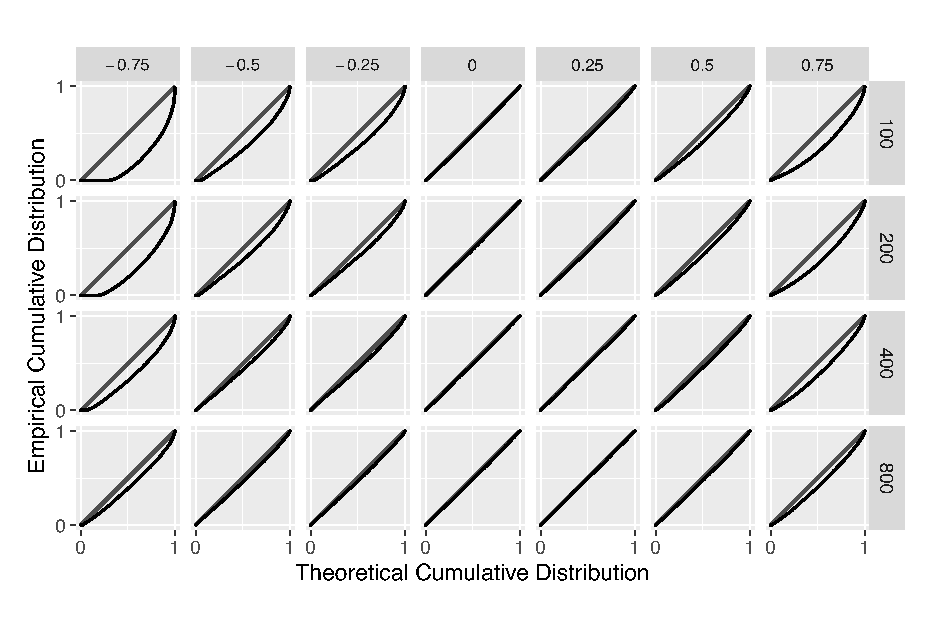
\includegraphics[width = .9\textwidth]{figures/alt_normal}
  \centering
  \vspace{-10pt}
  \caption{Q-Q plots of the p-values testing that a time series
    have marginal normal distribution with true data generating distribution
    being $N(8,8)$, when using \citet{politis2004automatic}'s procedure
    to select block sizes.}
  \label{fig:alt_qq_n}
    \hspace{3cm}
  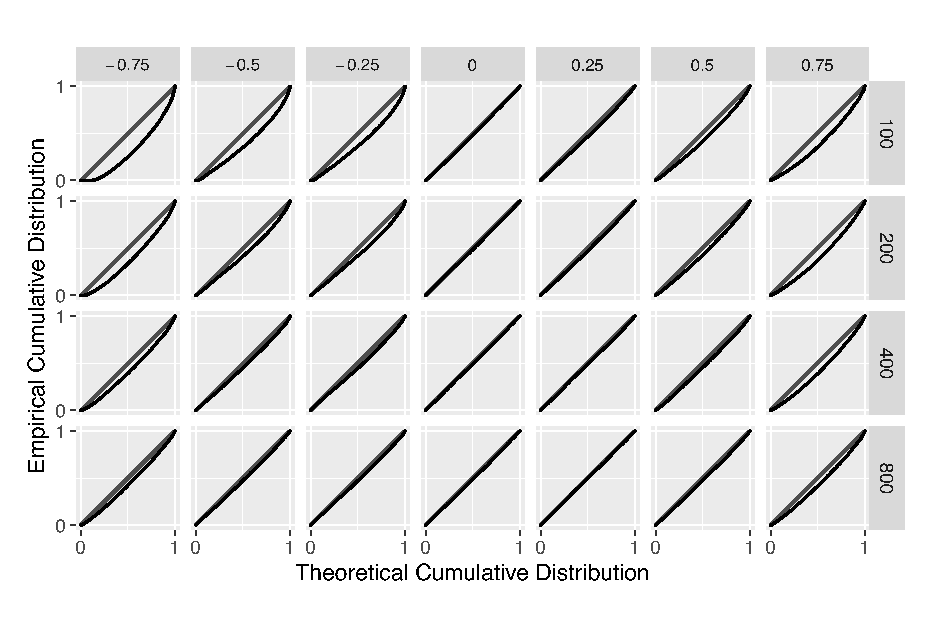
\includegraphics[width = .9\textwidth]{figures/alt_gamma}
  \vspace{-5pt}
  \caption{Q-Q plots of the p-values testing that a time series
    have marginal gamma distribution with true data generating distribution
    being $\Gamma(8,1)$, when using \citet{politis2004automatic}'s procedure
    to select block sizes.}
  \label{fig:alt_qq_g}
\end{figure}


\begin{figure}[tbp]
  \centering
  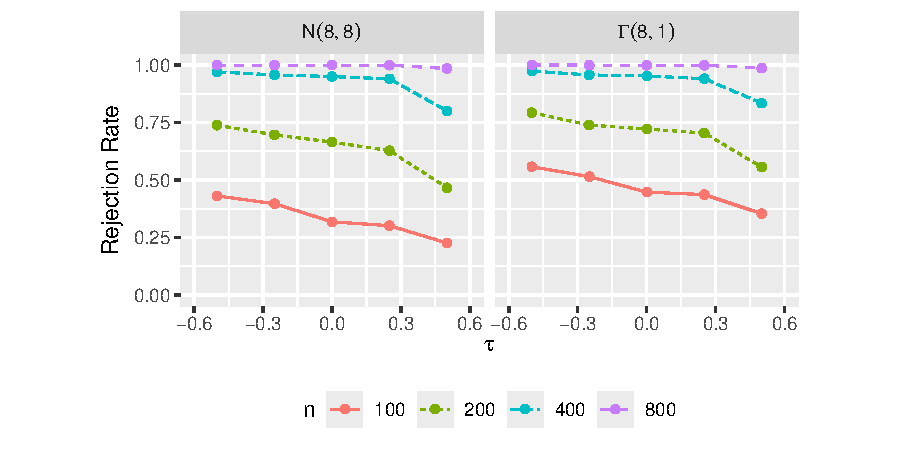
\includegraphics[scale=1]{figures/alt_rr}
  \caption{Empirical power curve as a function of $\tau$ for
    $n \in \{100, 200, 400, 800\}$ and true marginal distribution
    $\in \{N(8,8), \Gamma(8,1)\}$, when using \citet{politis2004automatic}'s 
    procedure
    to select block sizes. When the data was generated from $N(8,8)$,
    we tested for the gamma family. When the data was generated from
    $\Gamma(8,1)$, we tested for the normal family.
  }
  \label{fig:alt_rr}
\end{figure}


We evaluated the size and power performance of the NPBB test under automatic
block length selection. The size performance is shown
in Figures~\ref{fig:alt_qq_n} and \ref{fig:alt_qq_g}, which display Q-Q plots
of the $p$-values under the null for Normal and Gamma margins, respectively.
Recall from Figures~\ref{fig:qq_n} and \ref{fig:qq_g} that the cubic root 
setting holds its size quite well with small $n$ for $|\tau| \leq 0.25$,
whereas achieving nominal size for $|\tau| \geq 0.5$ require
$n > 200$, and for $|\tau| \geq 0.75$ require $n > 800$. The automatic
selection shows similar limitations for $|\tau| > 0.5$, where it does
not hold its size. Moreover, deviations from the diagonal line appear
larger for negative $\tau$, likely due to the high proportion of
occurrence of overly large block sizes. For example, while the cubic
root setting held its size well at $\tau = -0.25$ with small~$n$, the
automatic selection does not. At the same time, under $\tau = 0$ or
$\tau = 0.25$, the method with block size selected by
\citep{politis2004automatic} maintains reasonable size for moderately
positively dependent series.


Figure~\ref{fig:alt_rr} shows the power results under automatic selection.
When compared to Figure~\ref{fig:rr}, the two settings exhibit similar power
for $|\tau| \leq 0.5$, with the automatic selection sometimes yielding higher
rejection rates, particularly for smaller negatively dependent samples.
Overall, while the automatic selection from \citep{politis2004automatic}
performs reasonably well in certain settings, we recommend caution when using
it under negative~$\tau$ and smaller sample sizes, where maintaining nominal
size may be more difficult. In such cases, it may be sensible to apply a more
restrictive rule when setting the final block size---for example, using
$\min \{\sqrt{n}, \hat{l}\}$.


\bibliographystyle{asa}
\bibliography{citations}
\end{document}
